\documentclass[letterpaper]{article} % DO NOT CHANGE THIS
\usepackage[submission]{aaai2027}  % DO NOT CHANGE THIS
\usepackage[hyphens]{url}  % DO NOT CHANGE THIS
\usepackage{graphicx} % DO NOT CHANGE THIS
\urlstyle{rm} % DO NOT CHANGE THIS
\def\UrlFont{\rm}  % DO NOT CHANGE THIS
\usepackage{natbib}  % DO NOT CHANGE THIS AND DO NOT ADD ANY OPTIONS TO IT
\usepackage{caption} % DO NOT CHANGE THIS AND DO NOT ADD ANY OPTIONS TO IT
\frenchspacing  % DO NOT CHANGE THIS
\setlength{\pdfpagewidth}{8.5in} % DO NOT CHANGE THIS
\setlength{\pdfpageheight}{11in} % DO NOT CHANGE THIS
\usepackage{amsmath,amssymb,amsthm}
\usepackage{booktabs}
\usepackage{xcolor}
\pdfinfo{
/TemplateVersion (2027.1)
}
\setcounter{secnumdepth}{0}

\newtheorem{proposition}{Proposition}
\newcommand{\Ltriv}{L_{\mathrm{triv}}}
\newcommand{\kstar}{k^\star}

\title{Hemodynamic Attenuation: Pruning Attention Heads the Way the Brain Prunes Vessels}
\author{Anonymous Submission}
\affiliations{}

\begin{document}
\maketitle

\begin{abstract}
The brain keeps a blood vessel only while the flow it carries is worth its metabolic upkeep, and vessels that neighbours can cover regress gradually. We turn this principle into \emph{hemodynamic attenuation}, a rule that sizes a transformer's attention during training. Each head has a valve and pays a fixed upkeep. A head's value is the loss that would remain if it closed and the other heads re-fit to cover for it, the analogue of collateral flow. A head whose value falls below the upkeep is closed gradually, and a closed head reopens if it becomes valuable. No target size is set. The rule is greedy minimisation of loss plus upkeep, the form of Murray's law, so it makes predictions that can be checked before training. On a retrieval task whose minimal number of heads is known, the rule kept exactly that number in 29 of 30 runs and never broke the model, while three published pruning methods broke it in every run. In 36 further runs it kept that number at every upkeep below the threshold theory gives and collapsed to one head at every upkeep above it. Under random head failure on the same task it kept the number of backup heads predicted from a failure tree, 79 of 100 pre-registered runs exactly and all within one head, and the backups cut the loss under failure fivefold. It recovered the induction circuit in 10 of 10 runs. On GPT-2 small, across five samples of the published prompts, it found nested subsets of the published indirect-object circuit, from a 10-head core entirely inside it to 20--21 heads within one point of its accuracy.
\end{abstract}

\begin{figure*}[t]
\centering
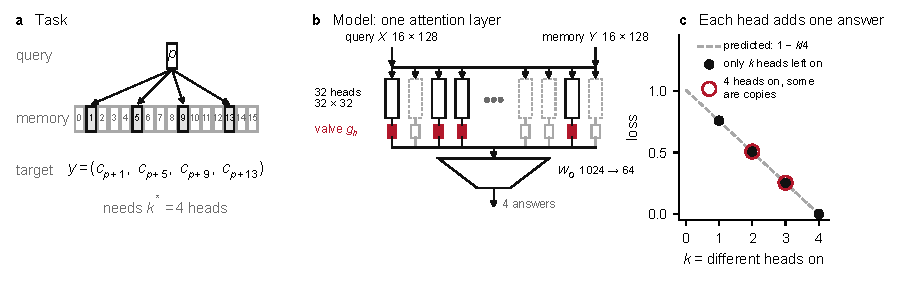
\includegraphics[width=\textwidth]{fig_task.pdf}
\caption{Hemodynamic attenuation on a task with a known minimal circuit. \textbf{(a)} A query names a position $p$; the target is the items at $R$ fixed offsets, here $R=4$, so 4 heads are needed. \textbf{(b)} Every head has a valve $g_h$ and pays a fixed upkeep while open. A head whose value, the loss its absence would cause after the others re-fit, falls below the upkeep is closed gradually (open: red; closed: grey). \textbf{(c)} Loss of a trained model with only $k$ heads on (black) follows $1-k/R$ (dashed). With 4 heads on, some of them copies, the loss is set by the number of \emph{different} heads (red): a copy is worth nothing. Units of $\Ltriv$.}
\label{fig:task}
\end{figure*}

\begin{figure}[t]
\centering
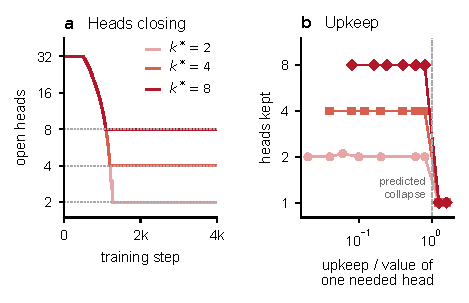
\includegraphics[width=\columnwidth]{fig_neuroai_col.pdf}
\caption{\textbf{(a)} Open heads during training, one run per task size; $\kstar$ dotted. \textbf{(b)} Heads kept against the upkeep, in units of the value of one needed head, $\Ltriv/R$. Theory predicts $\kstar$ heads left of 1 and one head right of it; 3 seeds per point.}
\label{fig:results}
\end{figure}

\begin{figure*}[t]
\centering
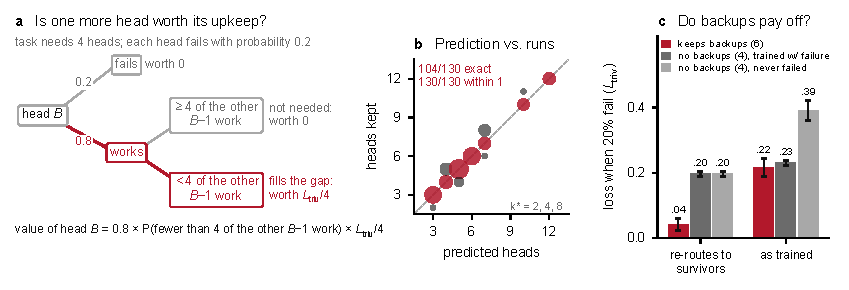
\includegraphics[width=\textwidth]{fig_backup_v2.pdf}
\caption{Backup heads, predicted from a failure tree. \textbf{(a)} Each head fails with probability $p$. An extra head is worth something only on one branch: it works and fewer than $\kstar$ others do, so it supplies the missing answer, worth $\Ltriv/\kstar$. \textbf{(b)} Heads kept against the prediction in all 130 damaged runs ($\kstar=2,4,8$, $p$ from 0.05 to 0.3, two upkeeps); dot size is the number of runs, red where exact. 100 of the runs were predicted in writing before they started (79 exact). \textbf{(c)} Loss when 20\% of the kept heads fail at test, 10 runs per arm, $\kstar=4$. With the read-out re-fitted to the survivors, the arm that kept backups loses five times less; as trained, training under failure gives most of the protection.}
\label{fig:backup}
\end{figure*}

\begin{figure*}[t]
\centering
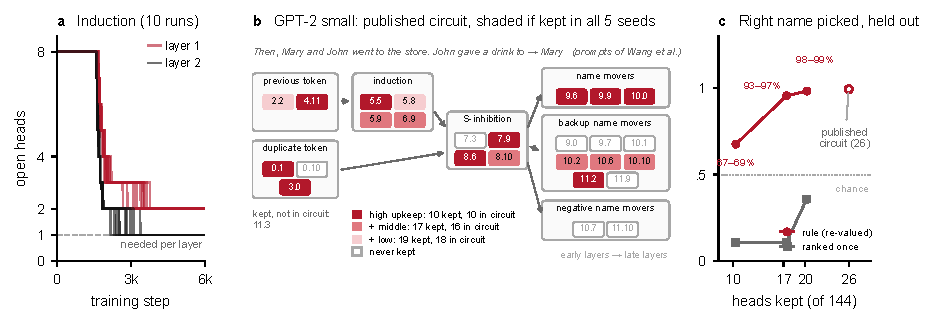
\includegraphics[width=\textwidth]{fig_circuits_v4.pdf}
\caption{Known circuits. \textbf{(a)} Induction, two layers of 8 heads: open heads per layer, 10 runs. Layer 2 closes to the one induction head. \textbf{(b)} GPT-2 small on indirect object identification, frozen weights, on the prompts of \citet{wang2023interpretability}. The 26 heads of the published circuit, grouped by the roles they assigned, from early to late layers. A head (layer.head) is shaded by the highest of three upkeeps at which our rule keeps it in all 5 seeds (different prompt samples); the sets are nested. The rule assigns no roles; it only decides which heads stay. \textbf{(c)} Held-out accuracy (1500 prompts per seed; bars span 5 seeds) against heads kept, for the rule and for the same number of heads ranked once against the full model, with the published circuit.}
\label{fig:circuits}
\end{figure*}

\section{Introduction}

A trained transformer usually has more attention heads than its task needs \citep{michel2019sixteen,voita2019analyzing}, and trained models keep backup heads that take over when others are removed \citep{wang2023interpretability,mcgrath2023hydra}. Existing pruning methods fix the final size by hand, as a target sparsity \citep{zhu2017prune}, a penalty strength \citep{voita2019analyzing,nam2025chg} or a threshold \citep{conmy2023towards}, and most prune after training, in one step. Regrowth during training \citep{evci2020rigging} is the closest precedent for reopening a head, but it too fixes the final sparsity. None decides how much redundancy to keep. And benchmarks with known circuits build the circuit in by construction \citep{lindner2023tracr,gupta2024interpbench}, so they cannot test whether a method finds the minimal circuit among the redundant heads that training produces.

The cerebral circulation solves a similar allocation problem without a target size. The neurovascular unit senses local demand and adjusts vessel diameter \citep{iadecola2017nvu}. Vessels that carry little flow regress gradually rather than being cut \citep{korn2015pruning}, and tissue survives the loss of a vessel when collaterals supply its territory. \citet{murray1926} showed that vessel size follows from minimising the work of moving blood plus the metabolic cost of keeping it: a vessel is kept only while it earns its upkeep.

We carry this principle over to attention heads (Table~\ref{tab:bio}). Our contributions are:
\begin{itemize}
\item \emph{Hemodynamic attenuation}, a rule that charges each head a fixed upkeep, values it by the loss that remains after the other heads compensate, and closes heads gradually during training, with reopening. It is greedy minimisation of loss plus upkeep (Proposition~1), so it makes predictions before training.
\item A benchmark whose minimal circuit, in size and roles, is known before training while the redundancy comes from training, with an exact loss law for $k$ heads.
\item Three predictions confirmed: the minimal head count on a benchmark where it is known, the upkeep at which the rule must collapse, and the number of backup heads under random failure.
\item Recovery of known circuits: induction, and a stable, nested core of the indirect-object circuit in GPT-2 small, which matches the published circuit with fewer heads.
\end{itemize}

\section{Hemodynamic Attenuation}

\begin{table}[t]
\centering
\small
\setlength{\tabcolsep}{4pt}
\begin{tabular}{@{}ll@{}}
\toprule
Cerebral vessels & Attention heads \\
\midrule
vessel, arteriole & head $h$, valve $g_h$ \\
metabolic upkeep (Murray) & upkeep $\pi$ per open head \\
collateral flow & other heads re-fit \\
unused vessel regresses & valve fades over 100 steps \\
flow returns with demand & closed head reopens \\
collaterals where occlusion likely & backups where failure likely \\
\bottomrule
\end{tabular}
\caption{The correspondence, a design principle rather than a model of blood flow.}
\label{tab:bio}
\end{table}

\paragraph{Valves.} Each head's output passes through a valve $g_h\in[0,1]$ before the heads are summed, $\hat{T}=\sum_h g_h\, O_h W_O^h$. A head with $g_h=0$ adds nothing and receives no gradient, so a model with $k$ open valves is exactly a $k$-head model.

\paragraph{Collateral value.} For the set $S$ of open heads, let $L^\ast(S)=\min_{W_O} L$ be the loss after the output weights of the heads in $S$ are re-fitted. The value of an open head is $v_h=L^\ast(S\setminus h)-L^\ast(S)$ and the gain of a closed head is $L^\ast(S)-L^\ast(S\cup h)$, both in closed form from the heads' output covariance. This is the Optimal Brain Surgeon score \citep{obs} for whole heads, as in ZipLM \citep{ziplm}; what is new is how it is used. If two heads output the same signal, the survivor takes over its twin's weight and the loss does not change, so a copy is worth nothing.

\paragraph{Schedule.} All valves start open. After a warm-up of 10\% of training, every 25 steps the rule closes the lowest-valued open head if $v_h<\pi$, and otherwise reopens the highest-gain closed head if its gain exceeds $2\pi$. A closing valve falls by $1/100$ per step, so a head regresses while the others adapt. The upkeep is $\pi=0.03\,\Ltriv$, where $\Ltriv$ is the loss of predicting the mean.

\paragraph{The rule optimises an objective.} Let $J(S)=L^\ast(S)+\pi|S|$, the loss plus the upkeep of the open heads, the form of Murray's cost. Every step of the rule lowers this one cost, so where the rule stops can be worked out before training.
\begin{proposition}
Closing $h$ lowers $J$ exactly when $v_h<\pi$, and reopening $h$ lowers $J$ by more than $\pi$. At a fixed point, no single removal lowers $J$ and no single addition lowers it by more than $\pi$. If needed heads are worth more than $\pi$ and redundant heads less, the fixed point keeps exactly the needed heads, for any such $\pi$.
\end{proposition}
The first two claims follow from $J(S\setminus h)-J(S)=v_h-\pi$ and $J(S\cup h)-J(S)=\pi-\mathrm{gain}_h$; since every step lowers $J$, the rule stops. It is forward--backward greedy selection \citep{pudil1994floating,zhang2011foba} over groups of weights, run while the heads are still learning. The proposition makes a falsifiable prediction: the number of heads kept should not depend on $\pi$ while $\pi$ lies between the value of a redundant head and that of a needed one, and should change abruptly outside that range.

\section{A Benchmark with a Known Minimal Circuit}

The task adapts sparse retrieval \citep{sanford2023representational} so that the number of heads, not the width, is the constraint. A memory of $N=16$ slots holds random items $c_j$, redrawn for every example. A query names a position $p$, and the target is the $R$ items at fixed offsets, $(c_{p+\delta_1},\dots,c_{p+\delta_R})$ (Figure~\ref{fig:task}a). A head returns one weighted average of the items, one linear combination of the $R$ unknowns, so $R$ items need $R$ heads with different attention patterns. With $k\le R$ such heads the lowest achievable loss is
\begin{equation}
L^\ast(k)=\left(1-k/R\right)\Ltriv ,
\label{eq:law}
\end{equation}
confirmed on trained models to within $0.003\,\Ltriv$ (Figure~\ref{fig:task}c). Each needed head is worth $\Ltriv/R$ and each copy $0$, so Proposition~1 predicts exactly $\kstar=R$ heads for any $\pi<\Ltriv/R$, and a collapse to one head above it. The model is one cross-attention layer with $H=32$ heads, width 128 and no MLP. The task is solved when the loss is below $0.02\,\Ltriv$. \emph{Exact count} means the open heads over the last 40\% of training equal $\kstar$; \emph{intact} means that once solved, the loss never rises above the bar.

\section{Results}

\begin{table}[t]
\centering
\footnotesize
\setlength{\tabcolsep}{1.6pt}
\begin{tabular}{@{}lllccc@{}}
\toprule
Method & When & Size set by & Pred. & Exact & Intact \\
\midrule
\textbf{Ours} & training, gradual & upkeep & yes & \textbf{29} & \textbf{30} \\
ZipLM-style & once + tune & target & -- & 24 & 0 \\
Michel et al. & after training & target & -- & 28 & 0 \\
$L_0$ gates (Voita) & in training & penalty & -- & 9 & 0 \\
CHG & after training & penalty & -- & \multicolumn{2}{c}{not run} \\
ACDC & after training & threshold & -- & \multicolumn{2}{c}{not run} \\
\midrule
\quad no fade & & upkeep & & 30 & 0 \\
\quad no re-fit (OBD) & & upkeep & & 2 & 30 \\
\quad random head & & upkeep & & 30 & 6 \\
\bottomrule
\end{tabular}
\caption{The same 30 runs ($\kstar=2,4,8$, 10 seeds each) for every method \citep{ziplm,michel2019sixteen,voita2019analyzing}. ZipLM uses the same score as ours, applied once. ZipLM and Michel et al.\ were given the true count. \emph{Pred.}: the size kept can be predicted before training. Causal head gating (CHG) \citep{nam2025chg} and ACDC \citep{conmy2023towards} are listed for how they set the size; they were not run here.}
\label{tab:methods}
\end{table}

\paragraph{Exact count without breaking the model.} The rule kept exactly $\kstar$ heads in 29 of 30 runs and never broke the model (Figure~\ref{fig:results}a, Table~\ref{tab:methods}). Three published methods, two of them given the true count, broke the model in every run. ZipLM uses the same score, so the difference lies in how the score is used. Removing one part of the rule at a time shows what each part does: without the fade the model broke, as a vessel cut rather than regressed; without the re-fit the rule valued copies and kept too many heads; with a random choice of head it broke in 24 of 30 runs. Deleting the closed heads leaves 6--25\% of the model's parameters (30\% on induction, below).

\paragraph{The upkeep does not set the size, until theory says it should.} Every upkeep from $0.01$ to $0.1\,\Ltriv$ gave the exact count. Above $\pi=\Ltriv/R$ every needed head costs more than it saves, so the rule should close down to one head. All 18 runs below this point kept exactly $\kstar$ heads and all 18 above it kept one (Figure~\ref{fig:results}b), with final losses $0.50$, $0.75$ and $0.875\,\Ltriv$, Equation~\eqref{eq:law} at $k=1$.

\paragraph{Backup heads, predicted.} If each head fails with probability $p$ at every step, the value of the $B$-th head is $v(B)=\frac{1-p}{R}\Pr[\mathrm{Bin}(B-1,1-p)<R]\,\Ltriv$, the product along one branch of a failure tree (Figure~\ref{fig:backup}a), a $k$-out-of-$n$ calculation from reliability theory \citep{barlow1965reliability}, and the rule should keep the largest $B$ with $v(B)\ge\pi$. The prediction has no free parameter. We committed predictions for 100 new runs before starting them, over $\kstar=2,4,8$, $p$ from 0.05 to 0.3 and two upkeeps. 79 matched exactly and all 100 were within one head (Figure~\ref{fig:backup}b); keeping $\kstar$ heads, or enough that $\kstar$ work on average, would match 4 and about 33. Most misses come from two settings that were off by one in every run, one of them flagged as borderline in advance. To test whether backups pay off, we trained models with failure and the rule (6 heads), with failure but valuing heads as if nothing failed (4), and without failure (4). With 20\% of heads failing at test and the read-out re-fitted, the loss was $0.04$ against $0.20\,\Ltriv$ (Figure~\ref{fig:backup}c). Without the re-fit the gain is small, because training under failure already teaches the read-out to cope.


\paragraph{Induction.} A two-layer attention-only model with $8+8$ heads was trained to continue a repeated sequence. Its known circuit is a previous-token head in layer 1 and an induction head in layer 2 \citep{olsson2022}. Cross-entropy has no closed-form re-fit, so here a head is valued by the loss without it. The rule kept $2+1$ heads with the expected roles in 10 of 10 runs and never broke the model (Figure~\ref{fig:circuits}a). The second layer-1 head is a backup, cutting errors on the repeat from 1 in 8 to 1 in 200. Switching off the layer-2 head dropped accuracy from 99.9\% to chance.

\paragraph{GPT-2 small.} We applied the rule to the 144 heads of GPT-2 small on indirect object identification (``Then, Mary and John went to the store. John gave a drink to'' $\to$ ``Mary''), whose 26-head circuit was found by hand \citep{wang2023interpretability}. The weights were frozen, so the rule is exactly the greedy minimisation of Proposition~1. Prompts come from the generator of \citet{wang2023interpretability}, 15 templates in both name orders; each of 5 seeds draws 300 prompts to choose heads and 1500 held-out prompts to test them. A closed head is replaced by its mean output on prompts with three different names, and the upkeep is a fraction (0.05, 0.02, 0.01) of the loss gap between all heads closed and all open. The rule kept 10--11, 17--18 and 20--21 heads at the three upkeeps, nested in every seed (Figure~\ref{fig:circuits}b). At the highest upkeep every head kept was in the published circuit; at the lower two, 94\%. Nineteen heads were kept in all 5 seeds, 18 of them in the circuit; the name movers were kept in all 15 runs and the negative name movers, which push against the correct name, in none. With 20--21 heads the rule picked the correct name in 98--99\% of held-out prompts, against 99.0--99.4\% for the published 26 heads and 99.1--99.8\% for the full model (Figure~\ref{fig:circuits}c). The upkeep acts as a dial that peels the circuit from its core outward. Re-valuing after every step matters. At 17--18 heads the rule picked the correct name in 93--97\% of prompts; the same number ranked once by their removal from the full model, in 8--13\%. The one-shot choice misses early duplicate- and previous-token heads, whose removal costs little while their backups are present but which the later heads need.

\section{Discussion}

The vascular principle that a vessel stays only while it earns its upkeep gives a pruning rule with no target size. It also gives an objective, and the objective predicts the count, the point of collapse and the number of backups before training.
\paragraph{Limitations.} The trained tasks are small and synthetic, chosen so that the minimal circuit is known. The proposition covers fixed heads; the fade and warm-up that handle learning heads are justified empirically. The backup count is shown on the benchmark only. In a first test on a character model trained on Shakespeare with whole heads failing at random (5 seeds), valuing heads under failure kept 1--3 more heads than valuing them without, as the tree predicts, but the number kept fell rather than rose as failure became more frequent; the model spreads its work across heads. Backups pay off mainly when the read-out can re-fit. On GPT-2 the weights were frozen, a single task was used, and we did not test how the kept heads perform on other tasks. Closed heads are still computed during training, so the compute saving is nominal until they are deleted.

\bibliography{refs}

\end{document}
